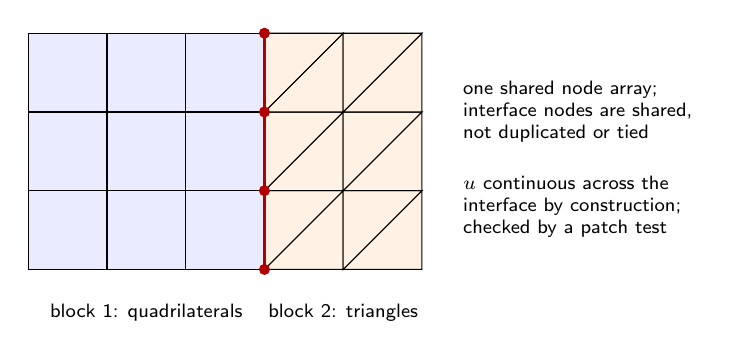
\begin{tikzpicture}[font=\sffamily\scriptsize]
\foreach \j in {0,1,2}{\foreach \i in {0,1,2}{ \draw[fill=blue!8] (\i*1.0,\j*1.0) rectangle ++(1,1);}}
\foreach \j in {0,1,2}{ \draw[fill=orange!10] (3,\j) -- (4,\j) -- (4,\j+1) -- cycle; \draw[fill=orange!10] (3,\j) -- (4,\j+1) -- (3,\j+1) -- cycle; \draw[fill=orange!10] (4,\j) -- (5,\j) -- (5,\j+1) -- cycle; \draw[fill=orange!10] (4,\j) -- (5,\j+1) -- (4,\j+1) -- cycle;}
\foreach \j in {0,...,3}{ \fill[red!70!black] (3,\j) circle (2pt);}
\draw[red!70!black,thick] (3,0) -- (3,3);
\node[align=center] at (1.5,-0.55) {block 1: quadrilaterals};
\node[align=center] at (4.0,-0.55) {block 2: triangles};
\node[align=left,anchor=west] at (5.4,2.0) {one shared node array;\\interface nodes are shared,\\not duplicated or tied};
\node[align=left,anchor=west] at (5.4,0.8) {$\bm u$ continuous across the\\interface by construction;\\checked by a patch test};
\end{tikzpicture}
